\documentclass[a4paper,12pt]{report}
\usepackage{algorithmic}
\usepackage[linesnumbered,ruled,vlined]{algorithm2e}
\usepackage[margin=2cm]{geometry}
\usepackage[utf8]{inputenc}
\usepackage{listings} 
\usepackage{graphicx} 
\usepackage{color}
\usepackage{xcolor}
\usepackage{hyperref}
\usepackage{verbatim}
%\usepackage{mdframed}

\newcommand{\currentdata}{14 February 2015}
\newtheorem{example}{Example}

\begin{document}
\vspace{-5cm}
\begin{center}
Department of Computer Science\\
Technical University of Cluj-Napoca\\
\includegraphics[width=10cm]{fig/footer}
\end{center}
\vspace{1cm}
%\maketitle
\begin{center}
\begin{Large}
 \textbf{Artificial Intelligence}\\
\end{Large}
\textit{Laboratory activity}\\
\vspace{3cm}
Name: Scutaru Lucian\\
Group: 30235\\
Email: lucianscutaru00@gmail.com\\
\vspace{12cm}
Teaching Assistant: Adrian Groza\\
Adrian.Groza@cs.utcluj.ro\\
\vspace{1cm}
\includegraphics[width=10cm]{fig/footer}
\end{center}

\tableofcontents

%\chapter{Rules and policies}
\newpage
\paragraph{Lab organisation.} 

\begin{enumerate}
 \item Laboratory work is 25\% from the final grade. 
 \item There are three deliverables in total: 1. Search, 2. Logic, 3. Planning.
%\item Tables~\ref{tab:first} and~\ref{tab:second} also bears out nine deadlines that you have to meet for achieving the points. They correspond to the following weeks: $W_2, W_4, W_5, W_6, W_{10}, W_{11}, W_{12}, W_{13}, W_{14}$. After each deadline you will get (or not) the achievable points. 
\item Before each deadline, you have to send your work (latex documentation/code) at moodle.cs.utcluj.ro

\item We use Linux and Latex
\item Plagiarism: Don't be a cheater! Cheating affects your colleagues, scholarships and a lot more.
\end{enumerate}
\begin{table}
\begin{center}
\caption{Lab scheduling}
\begin{tabular}{p{11cm}p{1.7cm}}\hline
\textbf{Activity} & \textbf{Deadline}  \\ \hline
{\it Searching agents, Linux, Latex, Python, Pacman}  & $W_1$ \\ %\hline
{\it Uninformed search} & $W_2$  \\ %\hline
{\it Informed Search} & $W_3$  \\ %\hline
{\it Adversarial search} & $W_4$ \\ %\hline
{\it Propositional logic} & $W_5$ \\ %\hline
{\it First order logic} & $W_6$ \\ %\hline
{\it Inference in first order logic} & $W_7$ \\ %\hline
{\it Knowledge representation in first order logic} & $W_8$ \\ %\hline
{\it Classical planning} & $W_9$ \\ %\hline
{\it Contingent, conformant and probabilistic planning} & $W_{10}$ \\ % \hline
{\it Multi-agent planing} & $W_{11}$ \\ %\hline
{\it Modelling planning domains} & $W_{12}$ \\ %\hline
{\it Planning with event calculus} & $W_{14}$ \\ \hline 
\end{tabular}
\end{center}
\label{tab:first}
\end{table}


\begin{comment}
\begin{center}
\begin{tabular}{ll}
Class: & Introducere in Inteligenta Artificiala\\
Enrollment key: & Iia2017-2018\\
\end{tabular}

\end{center}


\item {\it Laptop policy}: you can use your own laptop as long you have Linux. One goal of the laboratory is to increase your competency in Linux. It is \textbf{your} task to set static IPs:
\begin{center}
\begin{tabular}{ll}
IP: & 192.168.1.51\footnote{Or 52-59: avoid introducing the same IP for two different stations.}\\ 
MASK:&  255.255.255.0\\
GATEWAY:&  192.168.1.2\\
DNS:& 192.168.1.2\\
PROXY & 192.168.1.2:3128\\
\end{tabular}

Wifi:
\begin{tabular}{ll}
Network: &isg\\
Password: &inteligentaartificiala\\
\end{tabular}
\end{center}

\item {\it Group change policy.} Maximum number of students in a class is 14.

\item {\it For students repeating the class}: A discussion for validating the previous grade is mandatory in the first week. I usually have no problem to validate your previous grades, as long you request this in the first week. 
Failing to do so, leads to the grade 1 for the laboratory work in the current semester.
\end{comment}



\begin{comment}
\paragraph{Grading.}
Assessment aims to measure your knowledge and skills needed to function in realistic AI-related tasks.
Assessment is based on your written report explaining the nature of the project, findings, and recommendations. 
Meeting the deadlines is also important.
Your report is comparable to ones you would write if you were a consultant reporting to a client.

Grade inflation makes difficult to distinguish between students.
It also discourages the best students to do their best.
In my quest for ``optimal ranking of the students``, I do not use the following heuristics:

\begin{itemize}
 \item "He worked hard at the project``. 
Our society do not like anymore individuals that are $trying$, but individual that $do$ stuff.
Such heuristic is not admissible in education, except the primary school.

\item "I knew he could do much better". 
Such a heuristic is not admissible because it does not encourage you to spread yourself.
\end{itemize}

\begin{itemize}

\item 7 means that you: 
i) constantly worked during classes, 
 ii) you proved competent to use the tool and its expressivity for a realistic scenario, 
iii) you understood theoretical concepts on which the tool rely on.

\item 8, 9 mean that your code is large enough and the results proved by your experiments are significant.

 \item 10 means that you did very impressive work or more efficient 
that I expected or handled a lot of special cases for realistic scenarios.


\item 5 means that you managed to develop something of your own, functional, 
with your own piece of code substantially different from the examples available.

\item You obtain less than 5 in one of the following situations: 

\begin{enumerate}
\item few code written by yourself.
\item too much similarity with the provided examples.
\item non-seriosity (i.e. re-current late at classes, playing games, worked for other disciplines, 
poor/unprofessional documentation of your work, etc.)\footnote{Consider non-seriosity as a immutable boolean value that 
is unconsciously activated in my brain when one of the above conditions occurs for the first time.}.
\end{enumerate}

\item You get 2 if you present the project but fail to submit the documentation or code.
You get 1 if you do not present your project before the deadline.
You get 0 for any line of code taken from other parts that appear in section {\it My own code.} 
For information on TUCN's regulations on plagiarism do consult the active norms.

If your grade is 0, 1, or 2, you do not satisfy 
the preconditions for participating to the written exam. 
The only possibility to increase your laboratory grade is to take another project in the next year, 
at the same class, and to make all the steps again.   
\end{itemize}

However, don't forget that focus is on learning, not on grading.

{\it Using Latex in your documentation.} You have to show some competency on writing documentation in Latex. 
For instance, you have to employ various latex elements: lists, citations, footnotes, verbatim, maths, code, etc. 



\paragraph{Plagiarism.} Most of you consider plagiarism only a minor form of cheating.
This is far from accurate. Plagiarism is passing off the work of others as your own to gain unfair advantage. 

During your project presentation and documentation, 
I must not be left with doubts on which parts of your project are your work or not.  
Always identify both: 
1) who you worked with and 
2) where you got your part of the code or solution.
You should sign the declaration of originality. 

Describe clearly the starting point of your solution.
List explicitly any code re-used in your project. 
List explicitly any help (including debugging help, design discussions) provided by others (including colleagues or teaching assistant). 
Keep in mind that it is your own project and not the teaching assistant's project. 
Learning by collaborating does remain an effective method. 
You can use it, but don't forget to mention any kind of support. 
Learning by exploiting various knowledge-bases developed by your elder colleagues remain also an effective method for ''learning by example''. 
When comparing samples of good and poor assignments submitted by your colleagues in earlier years try to identify which is better and why. 
You can use this repository of previous assignments, but don't forget to mention any kind of inspiration source. 

The assignment is designed to be individual and to pose you some difficulties 
(both technological and scientific) for which you should identify a working solution by the end of the semester.  
Each semester, a distinct AI tool is assigned to two students. 
Your are encouraged to collaborate, especially during the the installation and example understanding phases ($W_1$-$W_4$). The quicker you get throughout these preparatory stages, the more time you have for your own project.


\paragraph{Class attendance.} 
I expect active participation at all activities. %We are all grown-ups, when and whether you attend lecture is up to you\footnote{However, you should be aware that when signing the study contract, you have some moral obligations towards the people that are paying your classes through the Ministry of Education budget.}. 
Keep in mind the exam can include any topic that was covered during class, explained on the board, 
or which emerged from discussions among participants. 
Missing lab assignments or midterm leads to minimum grade for that part.
You are free to manage your laboratory classes - meaning that you can submit the project earlier -  as long as you meet all the constraints and deadlines.
%However, it is mandatory to participate at the final public presentation of your project. 
\end{comment}

%\chapter{Laboratory works}

\chapter{A1: Introducere}

Am realizat doua domenii diferite cu ajutorul PDDL impreuna cu cate 4 probleme diferite pe care acesta le rezolva. Primul domeniu realizat se numeste Color Pipes si descrie regulile unui joc logic, in care utilizatorul trebuie sa conecteze punctele de aceeasi culoare, fara a intersecta liniile.\\
Cel de-al 2-lea domeniu mai complex descrie tot regulile unui joc numit Allout, in care scopul jucatorului este de a ajunge la stare in care tote luminile sunt stinse. Apasand pe ficeare din cele 25 de lumini asezate intr-o matrice, starea acestora se schimba(daca este deschis, becul se stinge), de asemenea luminile din jurul luminii apasate isi modifica starea.

\chapter{A2: Probleme si solutii}
\begin{Large}
 \textbf{       1. Color Pipes}\\
\end{Large}
Conecteaza punctele de aceeasi culoare pentru a trece la nivelul urmator. Tevile nu se pot intercala asa ca va trebui gasita o solutie astfel incat la final toate punctele de aceeasi culoare sunt conectate.\\

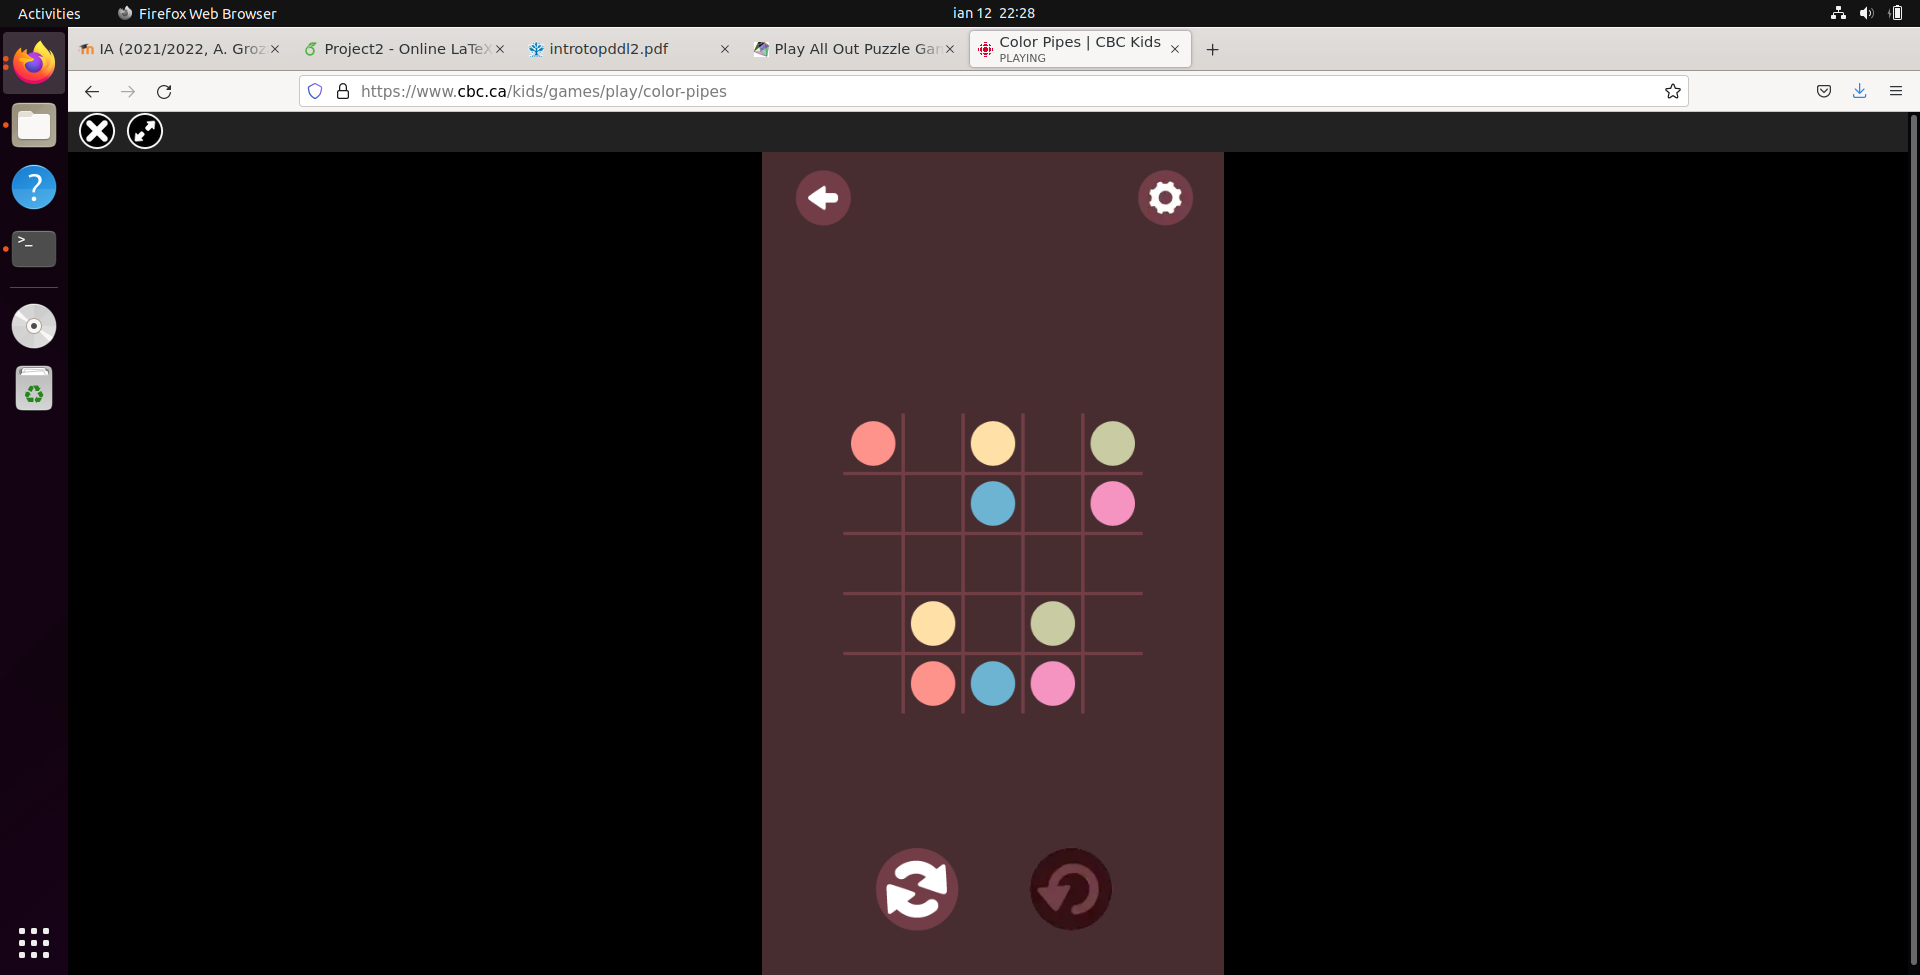
\includegraphics[width=150mm,scale=0.5]{pipes.png}\\
\begin{Large}
 \textbf{Rezolvare}\\
\end{Large}
In primul rand, in faza de dezvoltare a domeniului, ne definim predicatele de care avem nevoie. Cate un predicat pentru fiecare culoare diferita din joc, descris de locatie(rand si coloana). Consideram ca jocul se desfasoara pe o matrice patratica, deci ca si predicate vom avea nevoie si de coloanele si randurile adiecente celor curente. Astfel le luam ca si predicate.\\
In continuare, in cadrul domeniului descriem actiunile posibile pentru fiecare pipe(toate culorile). Pentru fiecare actiune ne luam ca si parametrii randul si coloana curenta, si in functie de caz randul sau coloana din partea de sus, jos, stanga sau dreapta a randului ci soloanei actuale. Ca si preconditii este suficient sa ne asiguram ca pipe-ul are culoarea pentru care descriem actiunea si in functie de miscare implementata, urmatorul rand/coloana sa fie descris.\\
Pentru partea de problema, luam ca si obiecte toate randurile sau coloanele din joc, si initializam jocul astfel. Descriem next-row si next-collumn pentru fiecare din randurile/coloanele din joc (avem nevoie doar de next pentru ca cu acesta putem lua si previous inversand in domain variabilele). Dupa care tot in initializarea jocului descriem punctele de inceput pentru fiecare culoare si in goal punem punctele la care fiecare trebuie conectate.\\
\\

\begin{Large}
 \textbf{2. Allout}\\
\end{Large}
Turn all the lights out, if you can!
Changing a light also changes the lights next to it.
Scopul jocului este ca toate luminile asezate initial intr-un grid de 5X5 sa fie stinse. Regulile jocului sunt simple. Cand apesi pe o lumina aceasta isi schimba starea(inchis-deschis) dar de asemenea si cele din jurul ei(axa X si Y) isi schimba starea.

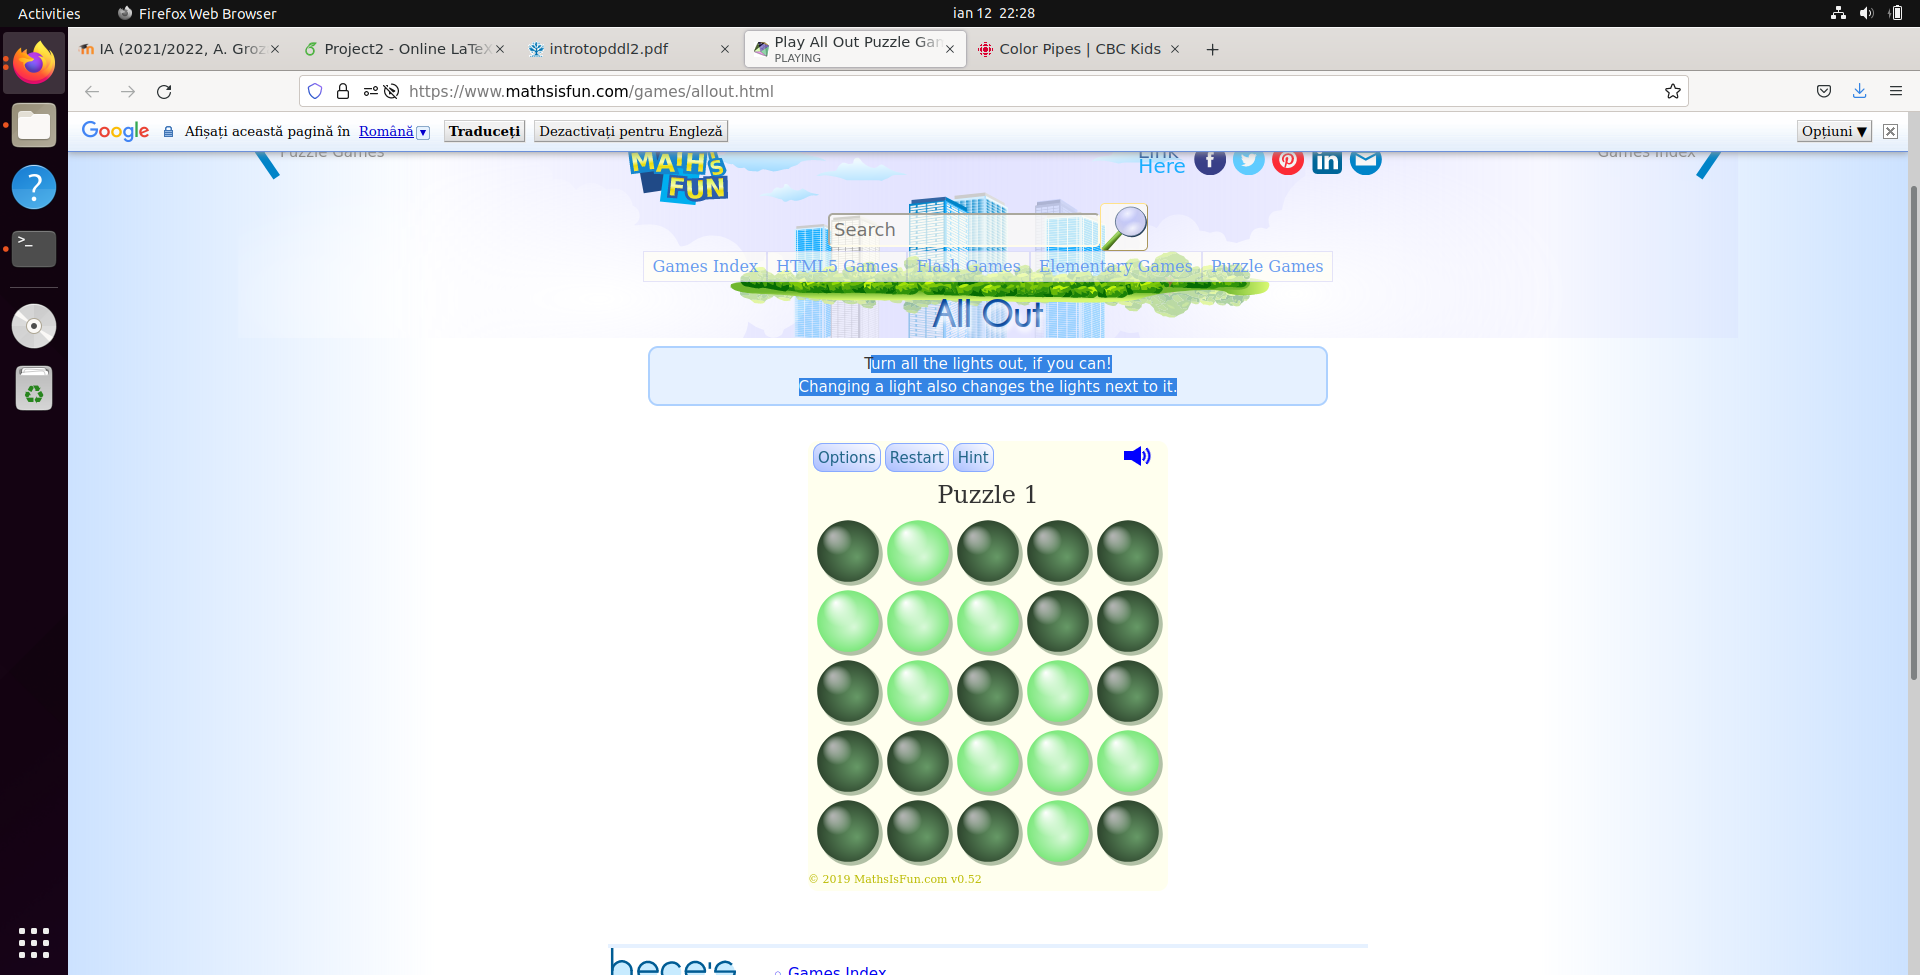
\includegraphics[width=150mm,scale=0.5]{out.png}\\
\begin{Large}
 \textbf{Rezolvare}\\
\end{Large}
In faza de dezvoltare a domeniului ne definim predicatele de care avem nevoie. In cazul de fata pentru rezolvarea problemei avem nevoie de un predicat pentru a descrie pozitia unei lumini(deschise sau nu), pozitia luminilor de la marginea gridului(pentru care regulile se modifica usor deoarece de exemplu pentru o lumina din coltul din dreapta sus, in cazul in care este pornita, numai lumina din stanga si cea de jos isi vor modifica starea. De asemenea, la fel ca si mai sus, luam ca predicate si randurile si coloanele adiacente.\\
In cadrul domeniului in continuare ne descriem actiunile. Deoarece exista multe cazuri de exceptie de la regula generala avem multe actiuni care sa trateza fiecare caz. Pentru luminile care nu se afla la marginea gridului implementam actiunea de pornire si oprire normala, dupa regula principala a jocului(se modifica si luminile din jurul lor), dar pentru luminile din margini tratam fiecare caz ca atare.\\
La partea de descriere a problemelor, ca si obiecte luam fiecare rand si coloana a jocului, descriem randurile si coloanele succesoare pentru fiecare dintre acestea, dupa care in initializarea jocului setam marginile gridului si punem coordonatele fiecarui punct de frontiera. Tot in initializare descriem ce lumini sunt pornite in momentul in care incepe jocul si in goal punem ca luminile de pe fiecare coloana si rand sa nu fie pornite.
\chapter{A3: Implementare}

%\input{mycode}
\begin{Large}
 \textbf{Color Pipes}\\
\end{Large}\\

 (:predicates\\
   (red ?r ?c)\\
   (green ?r ?c)\\
   (blue ?r ?c)\\
   (yellow ?r ?c)\\
   (pink ?r ?c)\\
   (next-r ?r ?r)\\
   (next-c ?c ?c)\\
  )\\
  Odata descrise predicatele trecem la implementare actiuilor. Fiecare culoare are ca si actiune move right/left/up/down. In continuare ca si exemplu am adaugat toate actiunile pe care pipe-ul de culoare roz le poate face.\\

(:action pink-up\\
    :parameters (?r ?c ?prev-r)\\
    :precondition (and (pink ?r ?c)\\
    			       (next-r ?prev-r ?r)\\
    			       (not (red ?prev-r ?c))\\
                       (not (green ?prev-r ?c))\\
                       (not (blue ?prev-r ?c))\\
                       (not (yellow ?prev-r ?c))\\
                )\\
    :effect (pink ?prev-r ?c)\\
  )\\

  (:action pink-down\\
    :parameters (?r ?c ?next-r)\\
    :precondition (and (pink ?r ?c)\\
    			       (next-r ?r ?next-r)\\
    			       (not (red ?next-r ?c))\\
                       (not (green ?next-r ?c))\\
                       (not (blue ?next-r ?c))\\
                       (not (yellow ?next-r ?c))\\
                )\\
    :effect (pink ?next-r ?c)\\
  )
  
  (:action pink-right\\
    :parameters (?r ?c ?next-c)\\
    :precondition (and (pink ?r ?c)\\
    			       (next-c ?c ?next-c)\\
    			       (not (red ?r ?next-c))\\
                       (not (green ?r ?next-c))\\
                       (not (blue ?r ?next-c))\\
                       (not (yellow ?r ?next-c))\\
                )\\
    :effect (pink ?r ?next-c)\\
  )  

  (:action pink-left\\
    :parameters (?r ?c ?prev-c)\\
    :precondition (and (pink ?r ?c)\\
    			       (next-c ?prev-c ?c)\\
    			       (not (red ?r ?prev-c))\\
                       (not (green ?r ?prev-c))\\
                       (not (blue ?r ?prev-c))\\
                       (not (yellow ?r ?prev-c))\\
                )\\
    :effect (pink ?r ?prev-c)\\
  )\\

\\



\begin{Large}
 \textbf{AllOut}\\
\end{Large}\\
  Dupa ce descriem predicatele trecem la implementare actiunilor. Initial descriem actiunile pentru fiecare din luminile din interiorul gridului(nu de pe margini). Dupa care tratam fiecare caz in parte pornind de la linia de sus a gridului, la liniile laterale si la fiecare colt.\\

(define (domain allOut)\\
(:predicates\\
	(light ?r ?c )\\
	(up ?r ?c)\\
	(down ?r ?c)\\
	(left ?r ?c)\\
	(right ?r ?c)\\
	(next-r ?r ?r)\\
	(next-c ?c ?c)\\
)\\

  (:action light-on\\
    :parameters (?r ?c ?prev-r ?next-r ?prev-c ?next-c )\\
    :precondition (and (not (light ?r ?c))\\
	    		(not (up ?r ?c))\\
	    		(not (down ?r ?c))\\
	    		(not (right ?r ?c))\\
	    		(not (left ?r ?c))\\
    			(next-r ?prev-r ?r)\\
    			(next-r ?r ?next-r )\\
    			(next-c ?prev-c ?c)\\
    			(next-c ?c ?next-c ))\\
    :effect (and (light ?r ?c) \\
    		(when (light ?prev-r ?c) (not (light ?prev-r ?c)))\\
    		(when (light ?next-r ?c) (not (light ?next-r ?c)))\\
    		(when (light ?r ?prev-c) (not (light ?r ?prev-c)))\\
    		(when (light ?r ?next-c ) (not (light ?r ?next-c )))\\
    		(when (not (light ?prev-r ?c)) (light ?prev-r ?c))\\
    		(when (not (light ?next-r ?c)) (light ?next-r ?c))\\
    		(when (not (light ?r ?prev-c)) (light ?r ?prev-c))\\
    		(when (not (light ?r ?next-c )) (light ?r ?next-c ))\\
		)\\
	)\\
	
\bibliographystyle{plain}
\bibliography{is}

1. IAlab-v1-1.pdf

2.https://www.latex-project.org/

3.https://www.cbc.ca/kids/games/play/color-pipes

4.https://www.mathsisfun.com/games/allout.html

\appendix

\chapter{Your original code}
Don't be a cheater! Cheating affects your colleagues, scholarships and a lot more.
This section should contain only code developed by you, without any line re-used from other sources. 
This section helps me to correctly evaluate your amount of work and results obtained. 


\vspace{2cm}
 
\begin{center}
Intelligent Systems Group\\
\includegraphics[width=10cm]{fig/footer}
\end{center}



\end{document}
